\documentclass{standalone}
\usepackage{tikz}
\usepackage{pgfplots}
\pgfplotsset{compat=1.18}
% Set background color
\pagecolor{gray!10} % Light gray background
\begin{document}
	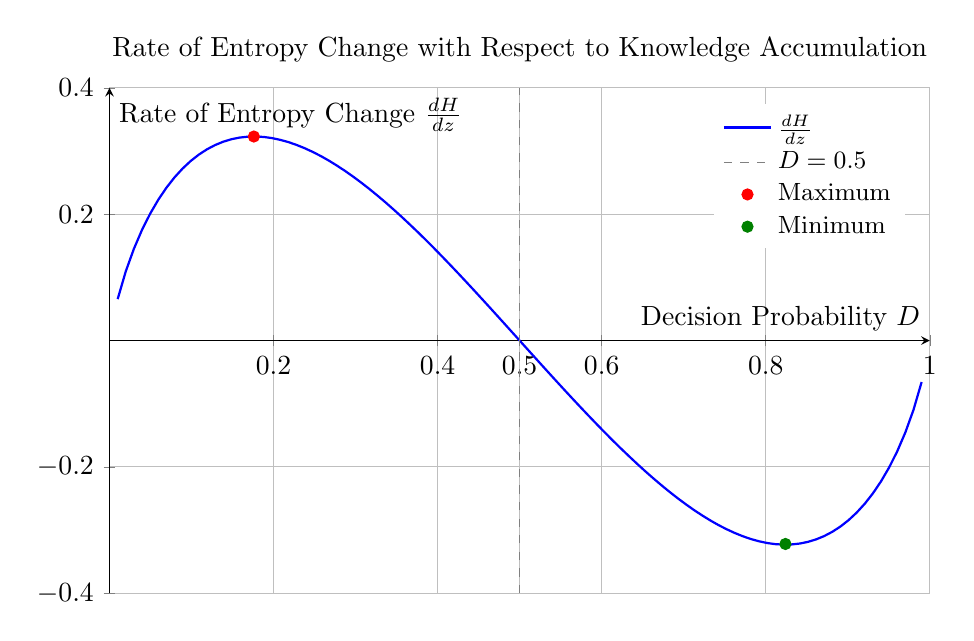
\begin{tikzpicture}
		\begin{axis}[
			width=12cm,
			height=8cm,
			xlabel={Decision Probability $D$},
			ylabel={Rate of Entropy Change $\frac{dH}{dz}$},
			title={Rate of Entropy Change with Respect to Knowledge Accumulation},
			grid=major,
			axis lines=middle,
			xmin=0,
			xmax=1,
			ymin=-0.4,
			ymax=0.4,
			xtick={0,0.2,0.4,0.5,0.6,0.8,1},
			ytick={-0.4,-0.2,0,0.2,0.4},
			legend pos=north east,
			legend style={
				draw=none,
				cells={anchor=west},
				font=\small
			},
			samples=100
			]
			
			% Main curve
			\addplot[
			thick,
			blue,
			domain=0.01:0.99,
			] {ln(1-x)/ln(2) * x * (1-x) - ln(x)/ln(2) * x * (1-x)};
			
			% Vertical line at D=0.5
			\addplot[
			gray,
			dashed
			] coordinates {(0.5,-0.4) (0.5,0.4)};
			
			% Maximum and minimum points
			\addplot[
			only marks,
			mark=*,
			mark size=2pt,
			red
			] coordinates {(0.1760,0.3230)};
			
			\addplot[
			only marks,
			mark=*,
			mark size=2pt,
			green!50!black
			] coordinates {(0.8240,-0.3220)};
			
			\legend{$\frac{dH}{dz}$, $D=0.5$, Maximum, Minimum}
			
		\end{axis}
	\end{tikzpicture}
\end{document}